%\chapter{Scraping}

% Resumir o capitulo aqui

%\subsection{Problem}
%\label{s:4_problem}
In most recent application, one of the most important components is data. As such, data classification is of utmost importance and each data source carefully selected. As a first step, we looke into some of the most common real-estate websites available in Portugal, compile into the following list:

\begin{itemize}
    \item \textbf{Idealista}: listing aggregator, fits all requirements but has advanced anti scraping mechanisms (i.e., captcha, ip blocking), as such it was avoided;
    \item \textbf{Imovirtual}: the second listing aggregator tried, provides reliable information that fits all criteria and is easy to scrape;
    \item \textbf{Remax}: It fits all requirements but unlike the previous websites, Remax is not a listing aggregator which results in a smaller number of listings;
\end{itemize}

Based on these platforms, we identified some of the core characteristics required to properly define a listing, and the following list represents the bare minimum listing detail required for the 15-Minute city platform.

\begin{itemize}
    \item \textbf{Location}: To be able to infer the distances between places having the location of each listing is mandatory. As such, these must include location names and coordinates;
    \item \textbf{Price}: It is one of the key limiting factors when searching for a new home, as such it is important to have the information available;
    \item \textbf{Size}: As pricing, it is relevant to understand the square meters of the house to decide if it is a good fit;
    \item \textbf{Bedrooms}: Number of rooms in each house excluding the kitchen and living room (following the Portuguese way of describing homes).
    \item \textbf{Commodities}: Perks associated with each house which may include: pools, garage, solar power, etc.
\end{itemize}

One of the most common occurrence between each website is the heavy reliance on Javascript, which makes them harder to scrape, one such example is the use of element rendering based on user interaction, where the host in orer to save bandwidth does not render the entire page until the user tries to use it. As such, specialized tools are required to simulate an user interacting with the application (e.g., scrolling down).

%With all of these in mind, we are now aware of what type of technologies we will need, and as such, the following section will go into detail of the tools at our disposal.

% Eescolher a informação necessária a extrair & fontes de informação
%The first obstacle was trying to understand the necessary data for the problem and, from there, how much of it is available. It was decided that the bare minimum information would be: Price, Location (Coordinates), Size (sqm), Bedrooms(T1,T2...) and Commodities. Therefore, while looking for sources, only the ones with that information would be considered. If a source also includes extra information such as the floor or textual descriptions of the house, the data is stored, which may allow for further analysis in the future, with techniques such as NLP. 

%Currently, there is several real estate companies that list AD information as required, the following websites were picked: Imovirtual, Idealista e Remax.

%As most of these websites are modern and rely heavily on Javascript, they require extra steps to allow data extraction, one example of those cases, is the use of element rendering based on user interaction, allowing the host do save bandwidth by not rendering the entire page. As such specialized tools are required to simulate an user interacting with the system (e.g., scrolling down).

% Falar da necessidade de obter dados de localizacao


\subsection{Solution}
\label{s:scraping-solution}

By defining the core characteristics necessary to describe each listing and analysing the needs of the systems, the first stop must be to defined the data model, which can be seen in Appendix \ref{apx:er-estates}. The model consists of two main categories: listing information and geographical data. The following listing contains a brief description of the main tables and their purposes:

\begin{itemize}
    \item \textbf{Estate}: listing information that describes each specific estate;
    \item \textbf{Feature}: possible features of a house such as garage, pool, etc;
    \item \textbf{Source}: know sources of where to scrape estate data;
    \item \textbf{Ad Status}: state of the listing;
    \item \textbf{Crawl History}: crawling occurrences of each listing;
    \item \textbf{Price History}: price evolution of a listing;
    \item \textbf{Location}: estate coordinates extracted from the scraped listing and associated with an estate;
    \item \textbf{Parish}: contains information that describes each civil parish, as well as their geographical properties (shape and centroid);
    \item \textbf{Municipality}: information that describes each municipality, as well as their geographical properties (shape and centroid);
    \item \textbf{District}: contains information that describes each district, as well as their geographical properties (shape and centroid);
    \item \textbf{Country}: information that describes each country, as well as their geographical properties (shape and centroid);
    \item \textbf{NUTS1}: NUTS \footnote{\textbf{N}omenclature of \textbf{T}erritorial \textbf{U}nits for \textbf{S}tatistics: is a geocode standard for referencing the subdivisions of countries for statistical purposes} 1 information and geographical properties (shape and centroid);
    \item \textbf{NUTS2}: NUTS 2 information and geographical properties (shape and centroid);
    \item \textbf{NUTS3}: NUTS 3 information and geographical properties (shape and centroid).
\end{itemize}

To store geographical data we opted to use a spatial database, which extends general purpose databases by providing spatial indexing and support for spatial queries. With it, it was possible to store geographic objects in vector formats, which allows effective and efficient management of geospatial data. Even though there were multiple solutions available to save this type of data, we chose PostGIS~\footnote{See: \url{https://postgis.net/}} a PostgresSQL extension, due to previous working experience.

This data was obtained through the \textit{OpenDataSoft}~\footnote{See: \url{https://www.opendatasoft.com/}} platform, which since then has been removed. While it was available it was possible to obtain the following portuguese data: districts, municipalities, parishes, NUT 2 and NUTS3. The geographical information pertaining the country and NUT1 information was not available. To fix it, we used spatial queries to intersect all the districts and merged into one polygon, representing the country of Portugal.

To extract the information from the chosen data sources, a scraping pipeline was first defined, as depicted in Fig. \ref{fig:scraping-architecture}. The goal was to create a solution that could easily be scaled to process different number of requests and also support the addition of new real estate websites to the pipeline.

\begin{figure}[H]
	\centering
	\begin{tikzpicture}
        \node{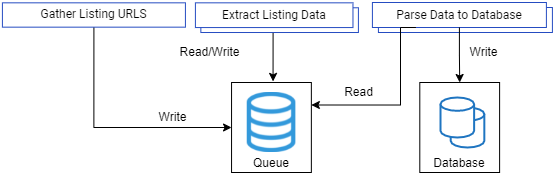
\includegraphics[width=1\linewidth]{Chapters/img/4_realEstateData/scraping-pipeline.png}};
        \node[xshift=-5cm, yshift=3cm, fill=white, circle, draw=gray]{1};
        \node[xshift= 0cm, yshift=3cm, fill=white, circle, draw=gray]{2};
        \node[xshift= 5cm, yshift=3cm, fill=white, circle, draw=gray]{3};
    \end{tikzpicture}
	
	\caption{Scraping architecture}
	\label{fig:scraping-architecture}
\end{figure}

This solution has three distinct sections, represented by three columns in Fig.~\ref{fig:scraping-architecture} where each has a different purpose:

\begin{enumerate}
    \item Responsible for gathering URLs and sending them to a queue named after their data source (e.g., remax-queue);
    \item Receive an URL from the queue, scrape the information from the listing and send it to the queue;
    \item Process the listings received by cleaning it and validating the information, then write it on the database;
\end{enumerate}

For the \textbf{first section}, it was necessary to obtain a base \acrshort{url} to act as a starting point for the scraper, which has to lead to a page with multiple estate listings. The goal was to get \acrshort{url}s that could provide as much data as possible, reducing the amount of pages scraped and avoiding overloading the source, while also trying to obtain listings for the entire country off of one \acrshort{url}. Which led to the following base \acrshort{url}s:

\begin{itemize}
    \item \textbf{Imovirtual}: https://www.imovirtual.com/comprar/apartamento/ ?search[order]= created\_at\_first:desc\&search[created\_since]=3 \&nrAdsPerPage=72
    \item \textbf{Remax}: https://remax.pt/comprar? searchQueryState= {"regionName":"", "sort": {"fieldToSort": "ContractDate","order":1}, "page":1, "mapIsOpen":false, "publishDate":7, "businessType":1, "listingClass":1}
\end{itemize}

For \textbf{Imovirtual}, to obtain the entire country with a single query, all it required was the deletion of the flag $&locations[0][region\_id]=ID$ and to obtain the maximum number of pages we had to include the flag \url{nrAdsPerPage=72}, being 72 the maximum number of listings possible to retrieve. In the \textbf{Remax} \acrshort{url}, we had to delete the information associated with the \textbf{\textit{regionName}} flag and send it as an empty string, as seen in the previous example. This way it was possible to retrieve the entire country all at once, however unlike Imovirtual it was not possible to tune the number of listings shown per page.

The third most important parameter in the \acrshort{url}s was the flag that allowed to query only listings published within certain time intervals. This way it was possible to schedule autonomous scraping through the use of CRON jobs, as it is possible to ensure we will retrieve all data published within the last days. Both of them impose no restrictions, as such it was possible to obtain the information for the entire year, but we decided to scrape them once a week to keep data fresh and only once week to not overload the hosts. The following flags were used: Remax -- \url{"publishDate":7} and Imovirtual -- \url{search[created_since]=7}.

To scrape the websites we opted to use \textbf{Scrapy} \footnote{See: \url{https://scrapy.org/}}, an established framework for large scale web scraping that provides all the tools to efficiently extract, process and store data while also being ready to be easily scalable and already organized into independent modules. One of the main workhorses of Scrapy are \textbf{Spiders}, the classes used to defined the custom behaviour for parsing the page(s). 

With the base \acrshort{url}s defined, we instructed the spider to process each page with the use of \acrshort{xpath}, which allowed us to extract the listings \acrshort{url}s, and send them to the queue. 

To provide a scalable experience, we opted to use a remote queue to act as an intermediary between all the components, as Scrapy was already prepared to use \textbf{Redis} and it was appropriate to the problem, it was chosen for this solution. Each item, was sent to a specific key according to their origin (\textit{remax:items} and \textit{imovirtual:items}), they were split into different categories as each website as different processing needs. After extracting all the listings from the first

The \textbf{second section} is responsible for extracting the actual listing data from each URL, which is obtained from the queue, and as before the data is extracted with the help of XPATH expressions. But, as stated previously, these websites only load elements through user interaction. To deal with this used \textbf{Selenium}, a framework commonly used for web application testing that has tools to automate and simulate human browsing behaviour. This was used in our advantage, by making the website think it is interacting with a user and allowing us to scrape the page content. This was possible by using the \textbf{Selenium Webdriver API} in conjunction with a browser driver (such as ChromeDriver for Google Chrome) and defining programmatic interactions through its library methods.

Imovirtual had this problem, where to extract the map coordinates it required the user to scroll down the entire page to load the map that showed the estate location.

The listing data is extracted, and mapped into a JSON composed of the following fields:

\begin{itemize}
    \item \textbf{URL} - URL of the ad;
    \item \textbf{Source} - Name of origin;
    \item \textbf{Price} - The current price of the estate;
    \item \textbf{Title} - Title of the ad;
    \item \textbf{Location} - Location name (district, municipality, parish), amount of fields varies based on the information provided and source;
    \item \textbf{Overview} - Must have estate information such as: square meters, floor, energy efficiency, bathrooms, etc...;
    \item \textbf{Description} - Textual description provided on the ad;
    \item \textbf{Features} - Extras included in the house (garage, lift, etc...);
    \item \textbf{Coordinates} - Longitude and Latitude;
    \item \textbf{Source Information} - Information provided by the source such as: id, date of creation and date of last modification.
\end{itemize}

Photos were excluded in the extraction as they were considered off limits as stated in the \textit{robots.txt} rules for each website. Each object is then sent into the queue \textit{general:processing}, which is now the same queue independent of source, so they can be processed by the next section of the pipeline. \\

During the \textbf{third section}, the items are now ready to be processed and inserted in the database. After the item is read from the queue, it gets sorted by the source name, and since each source has a corresponding function with the same name, it is possible to use Python reflection to call the appropriate function to process each item. This process can be observed in the following code: \\

\begin{lstlisting}[language=Java, caption={Snipet of code responsible for selecting the appropriate path for each item}, captionpos=t]
# Get JSON from the queue
json_str = self.redis.queue.blpop(self.queue_name)
# Extract item properties
item = json.loads(json_str[1].decode())['_values']
# Get the appropriate function from the source name received
method = getattr(self, item['source'], lambda: "Invalid source.")
# The method instantiates the required class to process the item 
selected_class = method(item, db_host, db_port)
# Start the cleaning process and obtain the final item
item = selected_class.main()
# Start process to insert onto the database
self.insertDB(item, selected_class)
\end{lstlisting}

During the event that occurs on line 10 of the previous code, all elements are processed which includes: removal of HTML tags, weird spacing, symbols (``€'' or ``$m^2$''), items in Portuguese are translated to English, etc. One of the most common problems were related to the locations, as due to user error, a large portion of the written locations described in the listings did not match the coordinates, sometimes even being in different continents, as such only items that had matching locations and coordinates were added to the database.

To validate this information, the coordinates obtained from the ad were intersected with the geographical information stored in the database, with the help of the ST\_WITHIN function from PostGIS, where we managed to obtain the real location name composed of: the parish, municipality, district, and country; and compare it with the information previously scraped.

During the fourth, and last step, items were stored in the database with the help of SQLAlchemy, an \acrfull{orm} -- a python library that translates Python objects to tables in SQL databases and automatically converts function calls to SQL statements (i.g., SQL \textit{WHERE} functions corresponds to filter\_by()). 

Since it is bound to happen that listings may appear multiple times, before each insertion, it is necessary to verify if the listing already exists in the database, if it does not, the object is created and promptly inserted. If they do exist, the items are instead updated as items such as house features, or textual descriptions may have been changed since the last time. Given that this process involves multiple tables and to ensure that data stays consistent all of this process is wrapped in a transaction that rolls back if any of the steps fails.

Due to the nature of the data, and its time relevancy (crawl history), every date and time reference is converted to the timezone of the server location (Europe/Lisbon) and converted to the ISO 8601 format (YYYY-MM-DDTHH:MM:SS), ensuring that everything is now consistent. \\

\subsubsection{Infrastructure}
\label{sss:scraping-infrastructure}

To deploy the previous pipeline, each process represented in Fig. \ref{fig:scraping-architecture} was containerized with Docker, always trying to keep the images as small as possible. All of them included the official Python image as our base image, instructions to copy our work directory and the dependencies installation. For processes that required selenium, we had to install chrome which is used by selenium to interact with the pages, which required the following configuration in the image dockerfile:

\begin{lstlisting}[float, language=Java, caption={Dockerfile configuration of the scrapper}, captionpos=t]
# Adding trusting keys to apt for repositories
RUN wget -q -O - https://dl-ssl.google.com/linux/linux_signing_key.pub | apt-key add -

# Adding Google Chrome to the repositories
RUN sh -c 'echo "deb [arch=amd64] http://dl.google.com/linux/chrome/deb/ stable main" >> /etc/apt/sources.list.d/google-chrome.list'

# Updating apt to see and install Google Chrome
RUN apt-get -y update
RUN apt-get install -y google-chrome-stable
# Installing Unzip
RUN apt-get install -yqq unzip

# Download the Chrome Driver
RUN wget -O /tmp/chromedriver.zip http://chromedriver.storage.googleapis.com/`curl -sS chromedriver.storage.googleapis.com/LATEST_RELEASE`/chromedriver_linux64.zip

# Unzip the Chrome Driver into /usr/local/bin directory
RUN unzip /tmp/chromedriver.zip chromedriver -d /usr/local/bin/
\end{lstlisting}

Given that each process now has their docker image, they could now be launched as Kubernetes deployments. \\

As the data extracted here is the most important to the project, we have tried to ensure that it would always be available. As such, the postgres cluster was deployed in a master-slave configuration with the help of \textbf{Bitnami PostgreSQL High-Availability}, a pre-existing package of \acrshort{k8s} configurations (helm charts) to deploy the cluster with minimal configuration.

Primary-secondary replication enables data from one database server (primary) to be replicated to one or more database servers (secondary). This way, database servers can work together to allow a secondary server to take over quickly if the primary server fails (high availability) with the use of the fail-over mechanism, or to allow several computers to serve the same data (load balancing).

\begin{figure}[H]
	\centering
	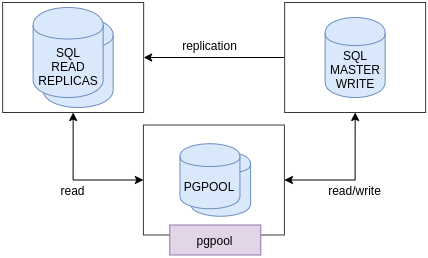
\includegraphics[width=0.7\linewidth]{Chapters/img/4_realEstateData/BD_Estates.png}
	\caption{Estates PostgreSQL architecture (Primary-Secondary)}
	\label{fig:bd-estates}
\end{figure}

These standby databases will remain synchronized with the primary node. The replication between the primary and the secondary nodes can be made via SQL statements or via internal data structure modifications. As this project used PostgreSQL, a stream of write-ahead log (WAL) records were used to keep the standby databases synchronized. WAL is a standard approach to transaction logging, where the main idea is that changes to the database must be written only after those changes have been logged. 


To effectively ensure high availability, it is not enough to have a primary-seconary architecture, so it is necessary to enable some automatic form of failover and since postgres does not have a default failover solution, PGPool-II was used. In this context, failover means automatically detaching PostgreSQL backend node which is not acessible by Pgpool. This inaccessibility is confirmed by regularly checking node healthiness, which it does by trying to connect to the node. When it happens, since the standby database contains all data of the main server, it can use it to become the new primary server. Unfortunately, even with all of this solutions data loss may still happen, since errors can occur in the middle of write operations and the logs for those operations may not had the time to be written. The cluster is then exposed to the outside via a \acrshort{k8s} service, represented with purple in Fig. \ref{fig:bd-estates}.

\begin{lstlisting}[float, language=Java, caption={Cron job specification to launch the scrapping jobs}, captionpos=t, label={lst:cronjob-configuration}]
apiVersion: batch/v1beta1
kind: CronJob
metadata:
  name: py-imovirtual-data-scale-up-cronjob
  namespace: py-scrapping
spec:
  successfulJobsHistoryLimit: 1
  failedJobsHistoryLimit: 1
  schedule: "0 0 * * 1" #Meia noite todas as segundas
  jobTemplate:
    spec:
      activeDeadlineSeconds: 180
      template:
        spec:
          serviceAccountName: scheduled-autoscaler-service-account
          containers:
          - name: py-imovirtual-urls
            image: biole/imoveis_scrapping:latest
            command: ["/bin/sh", "-c"]
            args: ['cd src; scrapy crawl imovirtual']
            resources:
              limits:
                memory: "400Mi"
                cpu: "300m"
            ports:
              - containerPort: 80
              - containerPort: 443
              - containerPort: 30036 
              - containerPort: 32658
          restartPolicy: Never
\end{lstlisting}


To handle the calendarization, scraping jobs were launched with \acrshort{k8s} using their own specification for \textbf{CronJobs}, as shown in listing \ref{lst:cronjob-configuration}. Within this configuration it is possible to configure the scheduling, so it occurs every seven days (every Monday at midnight), specify the container to run and arguments should it be run on. Additionally the pod resource usage was also configured, in this scenario the Memory and CPU usage was limited, letting the cluster know to never go below this values.




%As this section of the application contains the most important data , we have tried to ensure that it would always be available.
%As this was the most important section of data from the application, we tried to ensure it would always be safe and available.




% Falar aqui que sao dados importantes então base de dados tem backup, replicada, etc....


% Falar da infrastrutura necessária para ter tudo a funcionar (kubernetes): postgres, redis, python scripts
%% Falar dos recursos necessários (ex: foram atribuidos 200mb para o script X, 300mb para o y?)


